\documentclass[uplatex, 12pt, a4paper, dvipdfmx]{jsarticle}
\title{圏と層 斎藤毅\\講義ノート}
\author{司馬博文 J4-190549\\hirofumi-shiba48@g.ecc.u-tokyo.ac.jp}
\date{\today}
\pagestyle{headings}
\usepackage[top=15truemm,bottom=15truemm,left=10truemm,right=10truemm]{geometry}
\usepackage{amsmath, amsfonts, amsthm, mathptmx, amssymb, ascmac, amscd, color, comment, tikz-cd}
\newtheorem{theorem}{定理} \newtheorem{definition}{定義} \newtheorem{proposition}{命題} \newtheorem{corollary}[proposition]{系} \newtheorem{lemma}[proposition]{補題} \setcounter{secnumdepth}{4}
\begin{document}
\maketitle

\part{圏}
\section{集合と写像}
\begin{shadebox}\begin{definition}[集合]集合とは,物の集まり$X,Y$と,その元$x\in X$のことである.また,$X=Y$とは,$x\in X \Longleftrightarrow x \in Y$となることの略記である.$$\forall x,y \; [ \forall z (z\in x \Longleftrightarrow z\in y) \Longrightarrow x=y ] \hspace{3mm}\mathrm{(extentionality)}$$ \end{definition}\end{shadebox}
基本的にはZFC公理系によって集合を定義する.
\begin{shadebox}\begin{definition}[写像]写像とは,2つの集合$X,Y$について,$X$の各元$x$に対して$Y$の元$f(x)$が唯一つ定まっている時,$f$を$X$から$Y$への写像と呼び,$f:X\longrightarrow Y$で表す.\end{definition}\end{shadebox}
この$f$に対して,$X$を始域,$Y$を終域と呼ぶ.
なお,2つの写像$f,g:X\longrightarrow Y$が等しいとは,$f=g\Longleftrightarrow \forall x \in X \; [f(x)=g(x)]$と定められる.集合論の言葉で言えば「グラフが等しい」ことを,写像が等しいと定義する.
\begin{shadebox}\begin{definition}[写像の合成]2つの写像$f:X\longrightarrow Y, g:Y\longrightarrow Z$に対し,その合成写像$h:X\longrightarrow Z$が$\forall x \in X \; [h(x)=g(f(x))]$によって定めることができる.以降この$h$を$g\circ f$と書く.\end{definition}\end{shadebox}
\begin{shadebox}\begin{definition}[集合の積]2つの集合$X,Y$に対して,$X\times Y:=\{ (x,y) :\; x\in X \wedge y\in Y\}$と定義する.但し,$(x,y)=(x',y')\Longleftrightarrow x=x'\wedge y=y'$と定義する. \end{definition}\end{shadebox}
集合論的立場からは,$(x,y):=\{\{x\},\{x,y\}\}$と思えば良い.これを順序対,あるいは2-組という.
\begin{shadebox}\begin{definition}[写像の可換図式]$X,Y,W,Z$を集合とし,$f,g,h,k$を写像とする.以降$f:X\longrightarrow Y$を$X\xrightarrow{f}Y$とも書くこととする.この時,以下の図が可換図式であるとは,$h\circ f=k\circ g \Longleftrightarrow \forall x\in X \; [h\circ f(x)=k\circ g(x) \in W]\cdots\star^1$となることと定義する.
    $$ \begin{tikzcd}
        X \arrow[r, "f"] \arrow[d, "g"'] \arrow[dr, phantom, "\circlearrowright"] &  Y \arrow[d, "h"] \\
            Z \arrow[r, "k"] &    W \\
    \end{tikzcd} $$
\end{definition}\end{shadebox}
つまり,図式を有向グラフ(集合$X,Y,W,Z$を頂点,写像$f,g,h,k$を辺とした有向グラフ)だと思った時に,全ての有向道(directed path)が,写像の合成について,"等しい"(定義2の注釈参照)写像を与えるような図式を,可換図式という.「可換」であることの意味は強い,単に始域と終域が等しいだけでは足りない.\\
\textcolor{blue}{*図式の可換性は上のように定義した後,その集合論的な着地点$\star^1$を忘れ去ることが出来るはずだ.無理だろうか.}
\begin{shadebox}\begin{definition}[fiber積]終域が等しい2つの写像$f:X\longrightarrow S, g:Y\longrightarrow S$について,その\rm{fiber積}$X_f\underset{S}{\times_g}Y$を,$$X_f\underset{S}{\times_g}Y:=\{ (x,y)\in X\times Y:\; f(x)=f(y)\in S \}$$  \end{definition}\end{shadebox}
fiberとは(集合論で)単に逆像のことを意味する.2つの写像の,共通する終域$S$の各元$s$についての逆像$f^{-1}(s)=\{ x\in X:\; f(x)=s \},g^{-1}(s)$同士の積$f^{-1}(s)\times g^{-1}(s)$を,全ての$s\in S$について足し合わせたもの(和集合,或いは結びのこと)に他ならない.$$X_f\underset{S}{\times_g}Y=\bigcup_{s\in S}f^{-1}(s)\times g^{-1}(s)$$

\section{圏の定義}
\begin{shadebox}\begin{definition}[圏]圏とは,集合$C,M$と写像$s,t,c,e$の6-組$(C,M,s,t,c,e)$であって,図\ref{def-cd:1} \ref{def-cd:2} \ref{def-cd:3} \ref{def-cd:4}の可換図式を充たすもののことである.但し,$s,t,c,e$は夫々,\begin{eqnarray*}s:M\longrightarrow C,\hspace{5mm} t:M\longrightarrow C, \hspace{5mm} e:C\longrightarrow M\\[3mm] \left. 
\begin{array}{ccc}
    c:M_s\underset{C}{\times_t}M & \stackrel{c}{\longrightarrow} & M \\
    \rotatebox{90}{$\in$} & & \rotatebox{90}{$\in$} \\
    (g,f) & \longmapsto & c(g,f)
\end{array} \right. \hspace{10mm} \end{eqnarray*}を充たす写像である.

\vspace{1mm} \end{definition}\end{shadebox}

\begin{figure}[ht] \begin{center}  \caption{\label{def-cd:1} 集合論的に言えば,$s(f)=s(c(g,f))\wedge t(g)=t(c(g,f))$を表す可換図式.}
    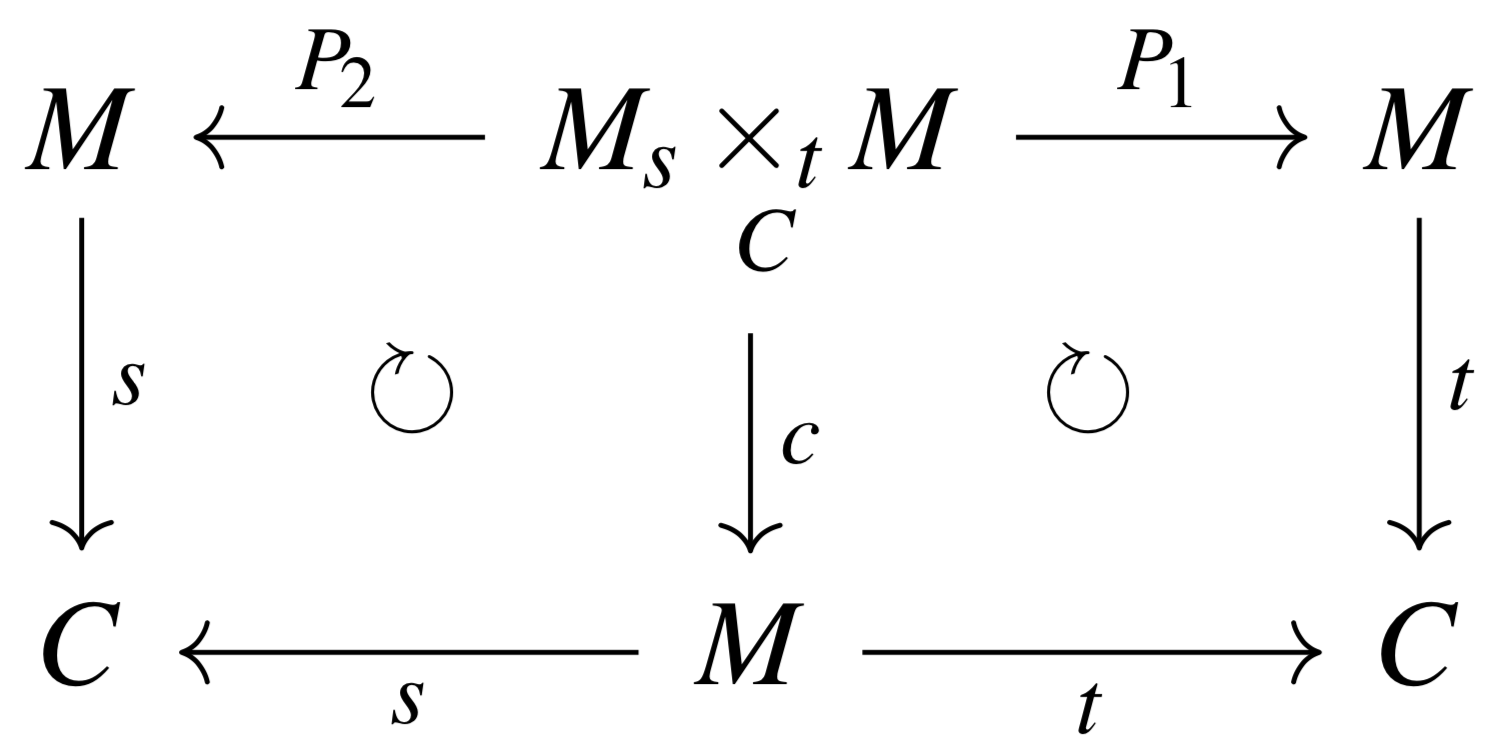
\includegraphics[width=7cm]{cd-1.png}
\end{center}\end{figure}
以降この$P_1, P_2$のことを射影と呼ぶ.\hspace{6mm}$P_1: X\underset{S}{\times}Y \longrightarrow X, \; \; \; P_2: X\underset{S}{\times}Y \longrightarrow Y$

\begin{figure}[ht] \begin{center}  \caption{\label{def-cd:2} 集合論的に言えば,$c(c(h,g),f)=c(h,c(g,f))$(射の合成についての結合則の成立)を表す可換図式.}
    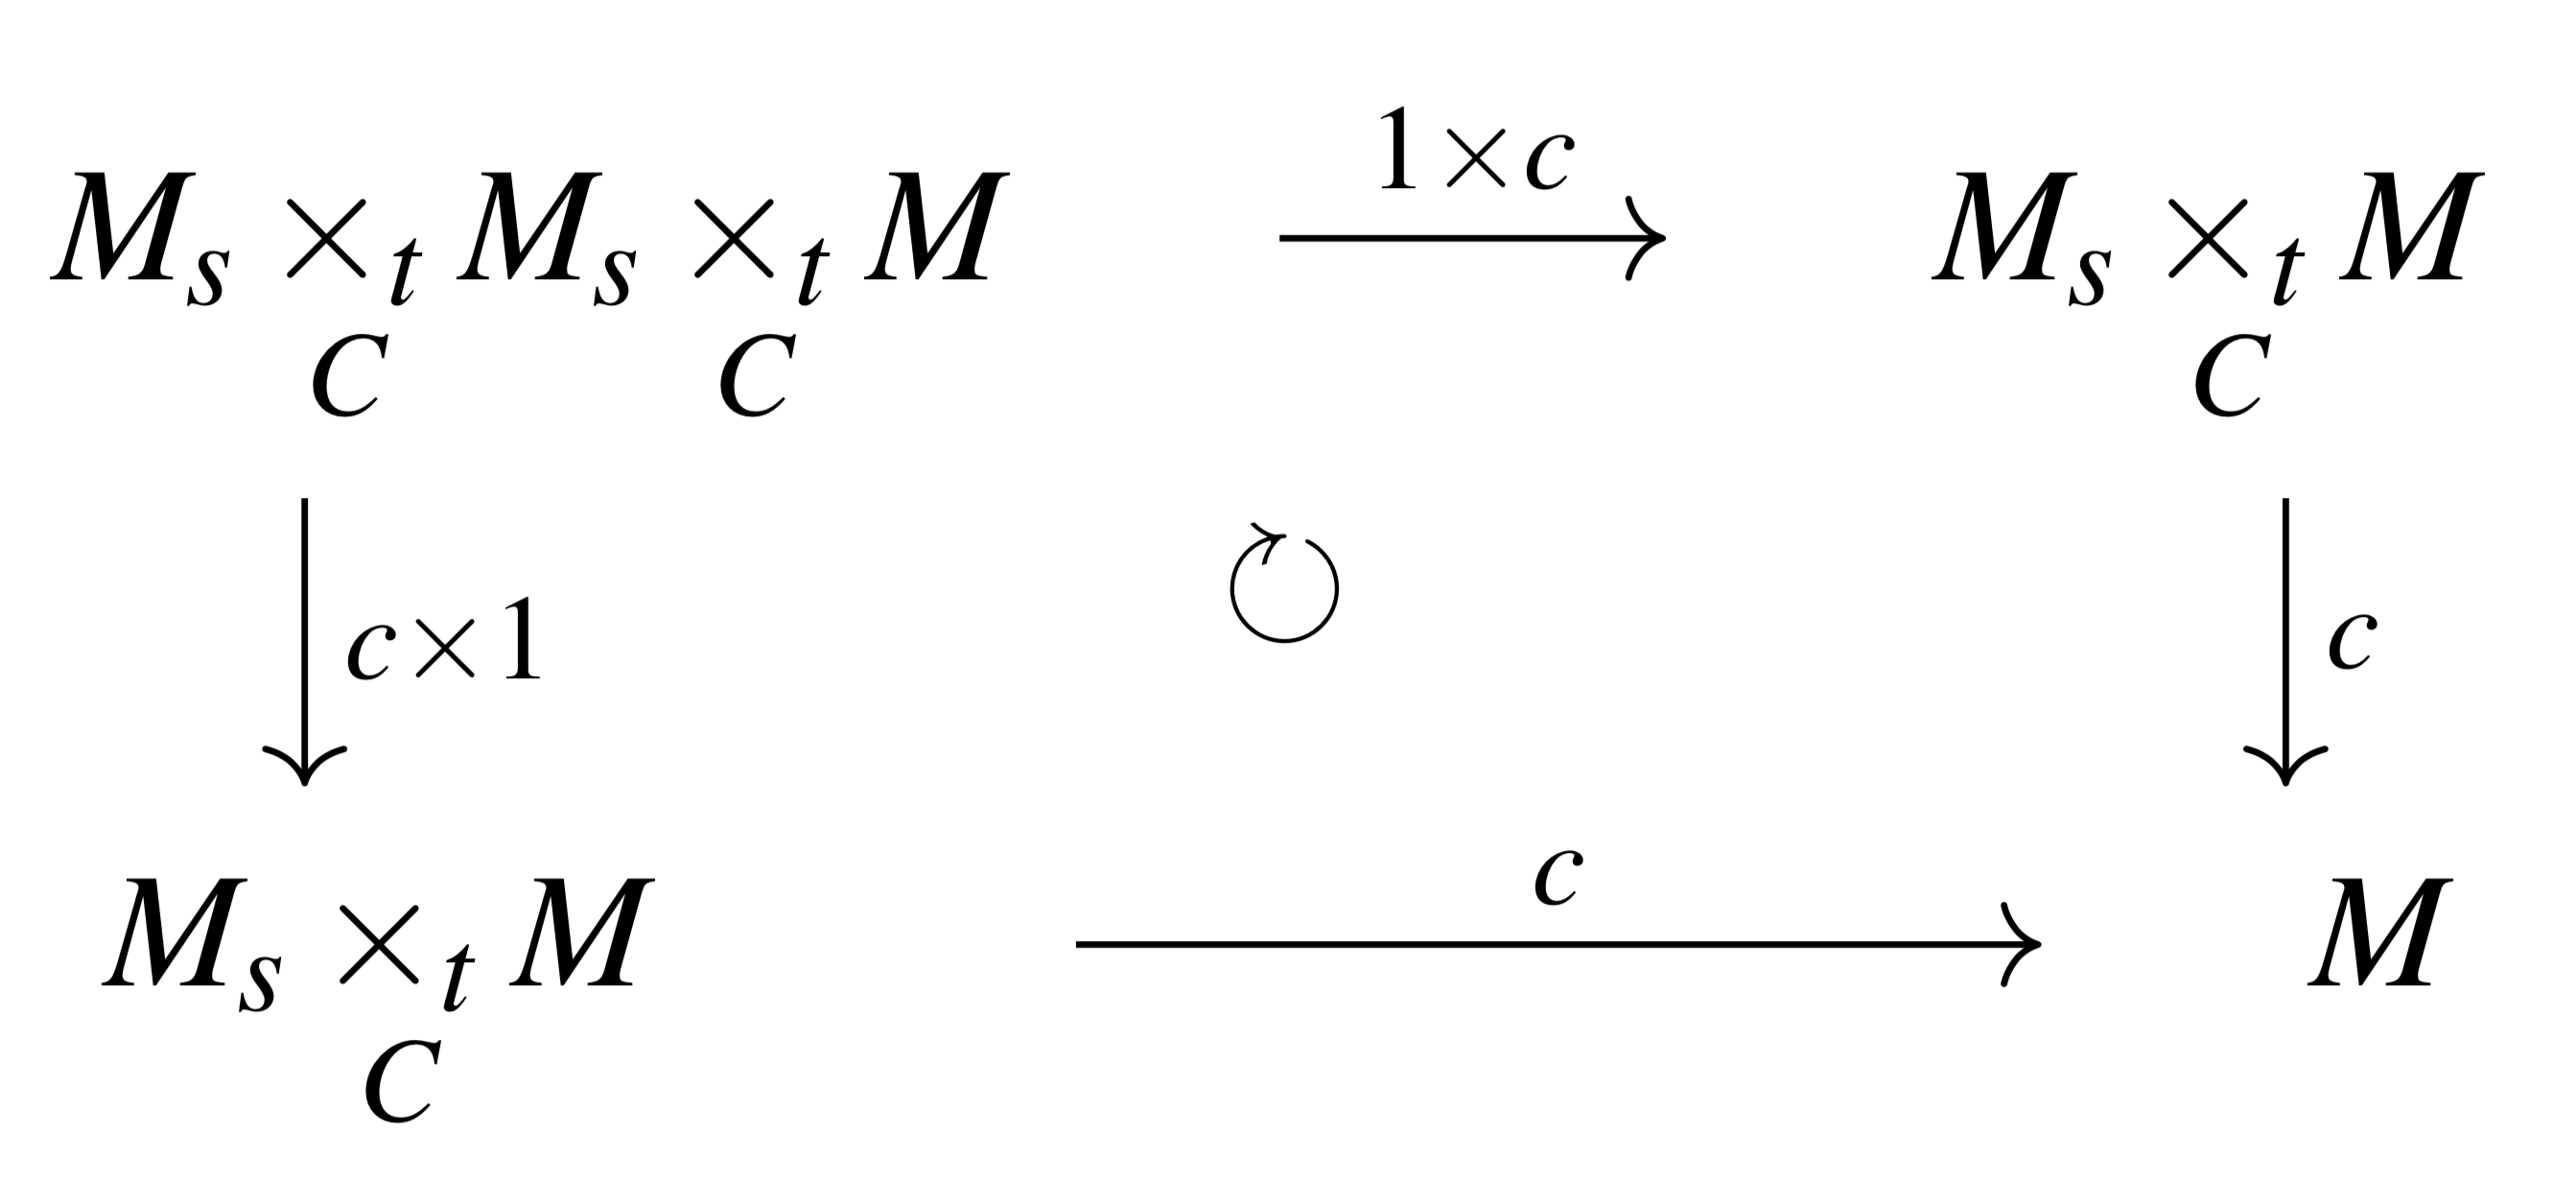
\includegraphics[width=7cm]{cd-2.png}
\end{center}\end{figure}
但し,$M_s \underset{C}{\times_t}M_s \underset{C}{\times_t}M := \{ (h,g,f)\in M\times M\times M : \; s(h)\overset{c}{=} t(g) \wedge \; s(g) \overset{c}{=} t(f) \}$であり,$$\begin{array}{ccc}
        c\times1:M_s\underset{C}{\times_t}M_s\underset{C}{\times_t}M & \longrightarrow & M_s\underset{C}{\times_t}M \\
        \rotatebox{90}{$\in$} & & \rotatebox{90}{$\in$}\\
        (h,g,f) & \longmapsto & (c(h,g),f) \\[3mm]
        1\times \! c:M_s\underset{C}{\times_t}M_s\underset{C}{\times_t}M & \longrightarrow & M_s\underset{C}{\times_t}M \\
        \rotatebox{90}{$\in$} & & \rotatebox{90}{$\in$}\\
        (h,g,f) & \longmapsto & (h,c(g,f))
\end{array}$$

これがwell-definedである理由は,図\ref{def-cd:1}より,$s(g)=s(c(h,g))=t(f)$が保証されているから,$(h,g,f)$は確かに必ず$M_s \underset{C}{\times_t}M_s \underset{C}{\times_t}M$に含まれるのである.\\[3cm]

\begin{figure}[ht] \begin{center}  \caption{\label{def-cd:3} 4つの写像について,$s\circ e=1_c=t\circ e$の関係を表す可換図式.}
    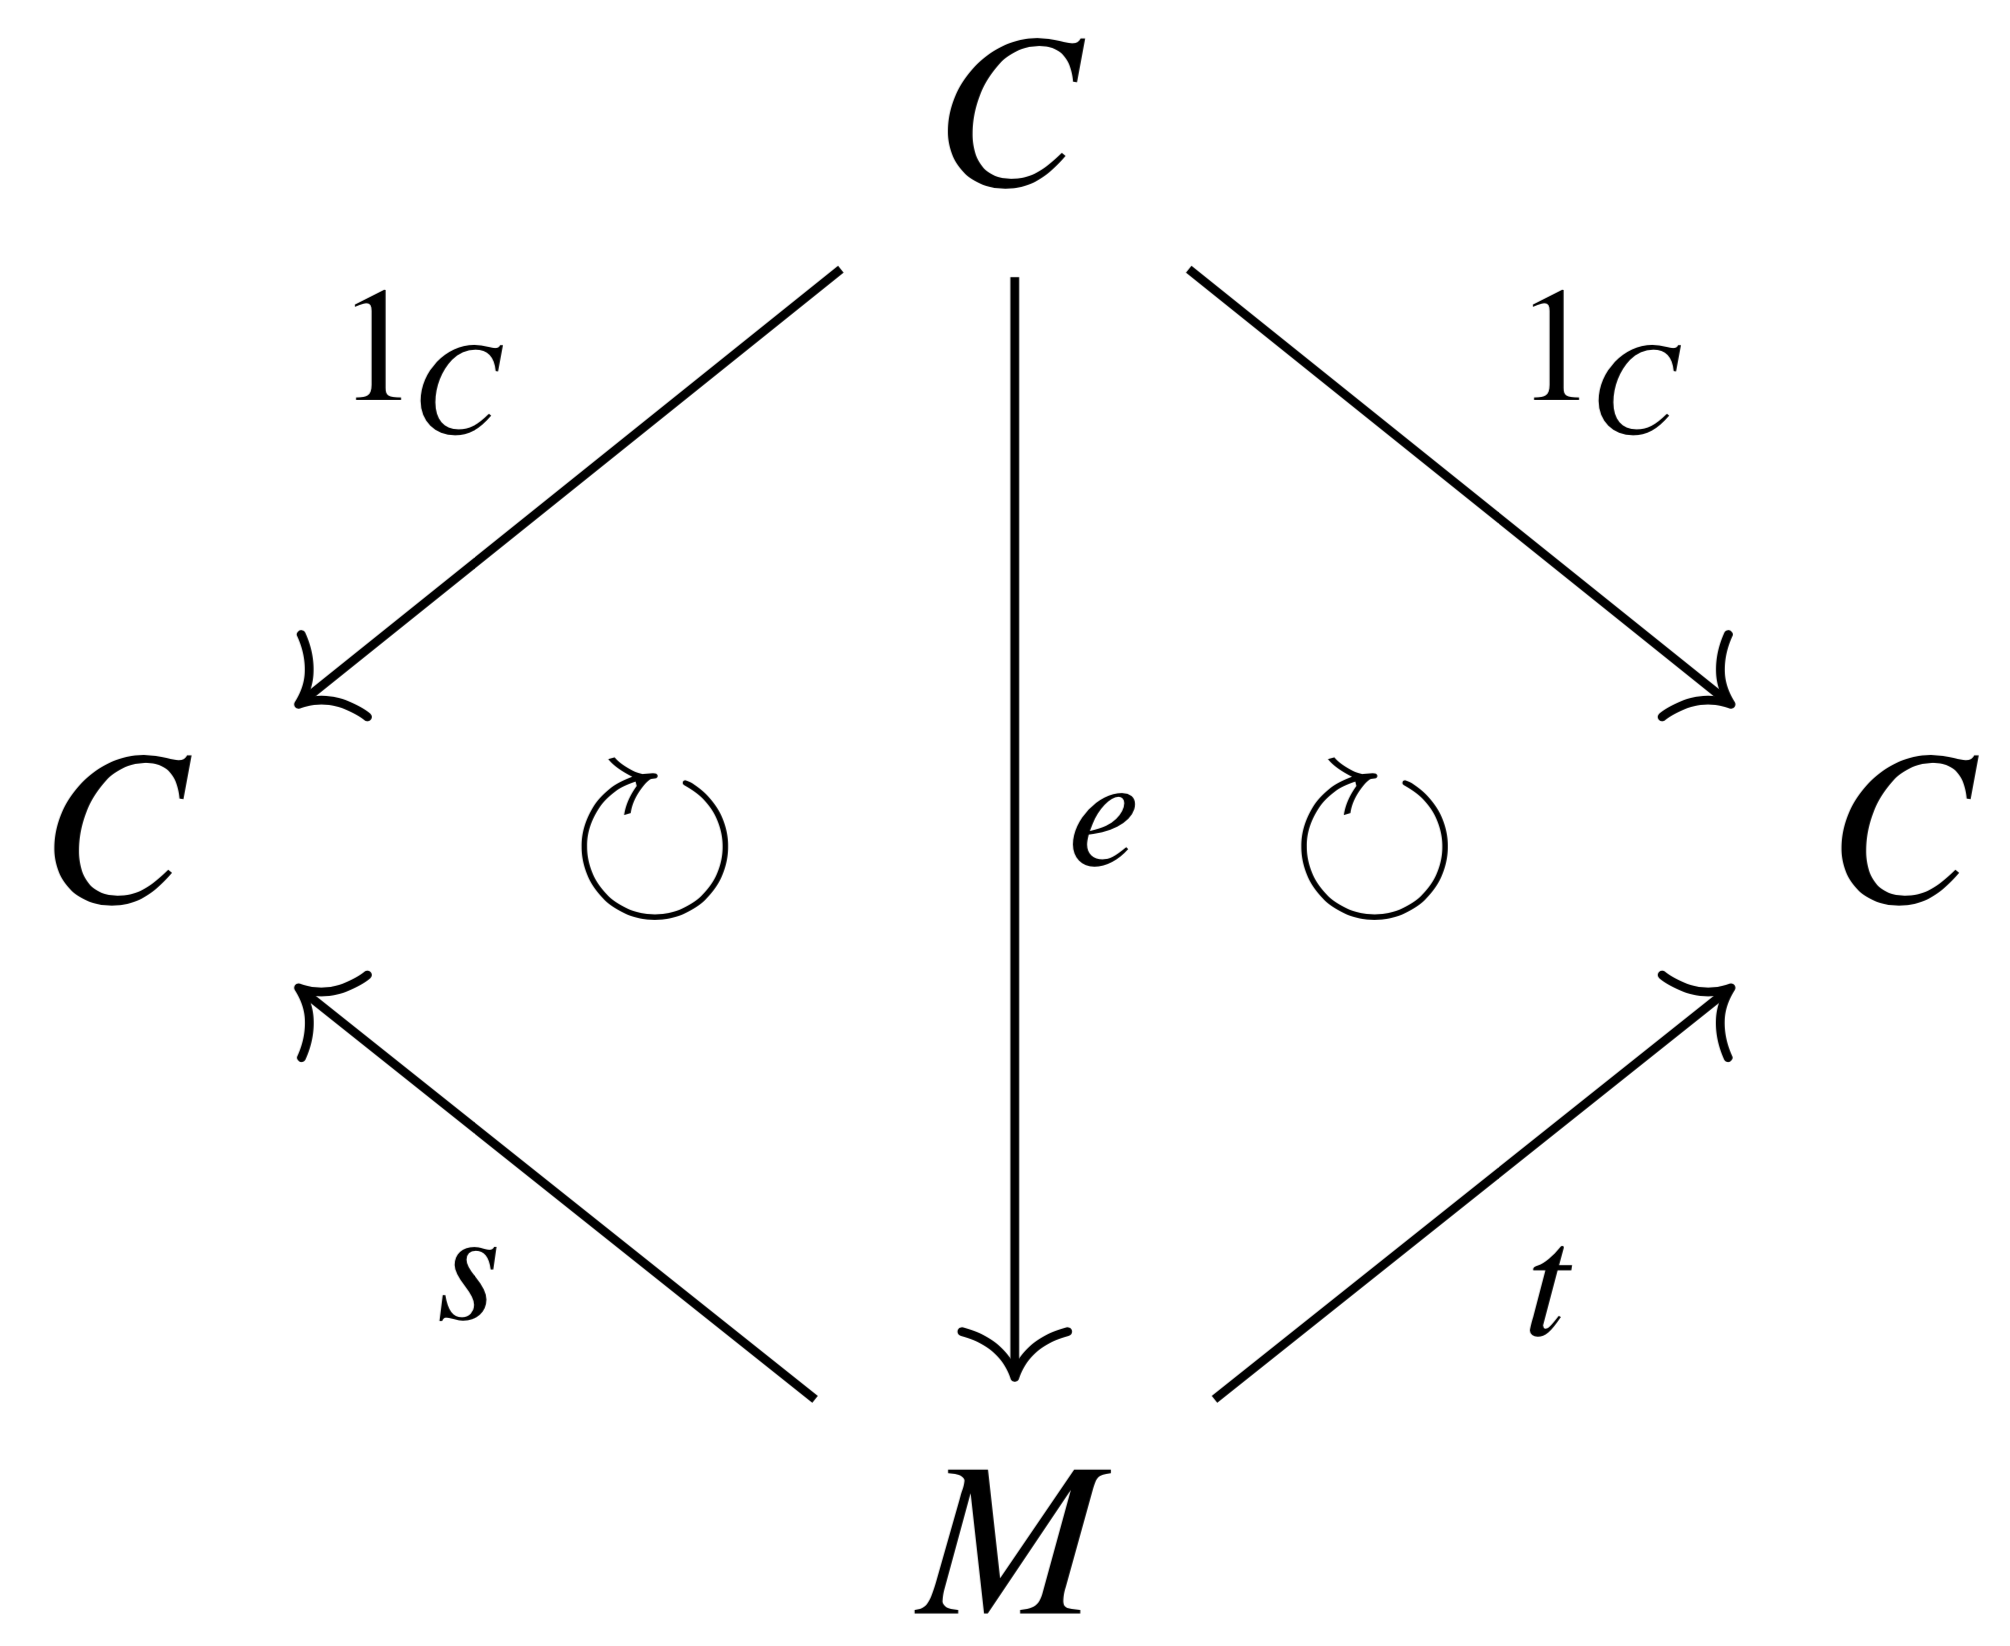
\includegraphics[width=7cm]{cd-3.png}
\end{center}\end{figure}
つまり,$C$の任意の元を$A$と取ると,$A=1_c(A)=s(e(A))=t(e(A))$だから,つまり,射$e(A)$は$e(A):A\longrightarrow A$である.このような射を恒等射と呼び,図\ref{def-cd:3}によると全ての$C$の元について定まる.

\begin{figure}[ht] \begin{center}  \caption{\label{def-cd:4} $c(e(t(f)),f)=c(f,e(s(f)))$即ち$f:A\longrightarrow B$と置いた時に,$f\circ e(A)=e(B)\circ f$(恒等射$e(A)$の特徴付け)を表す可換図式.}
    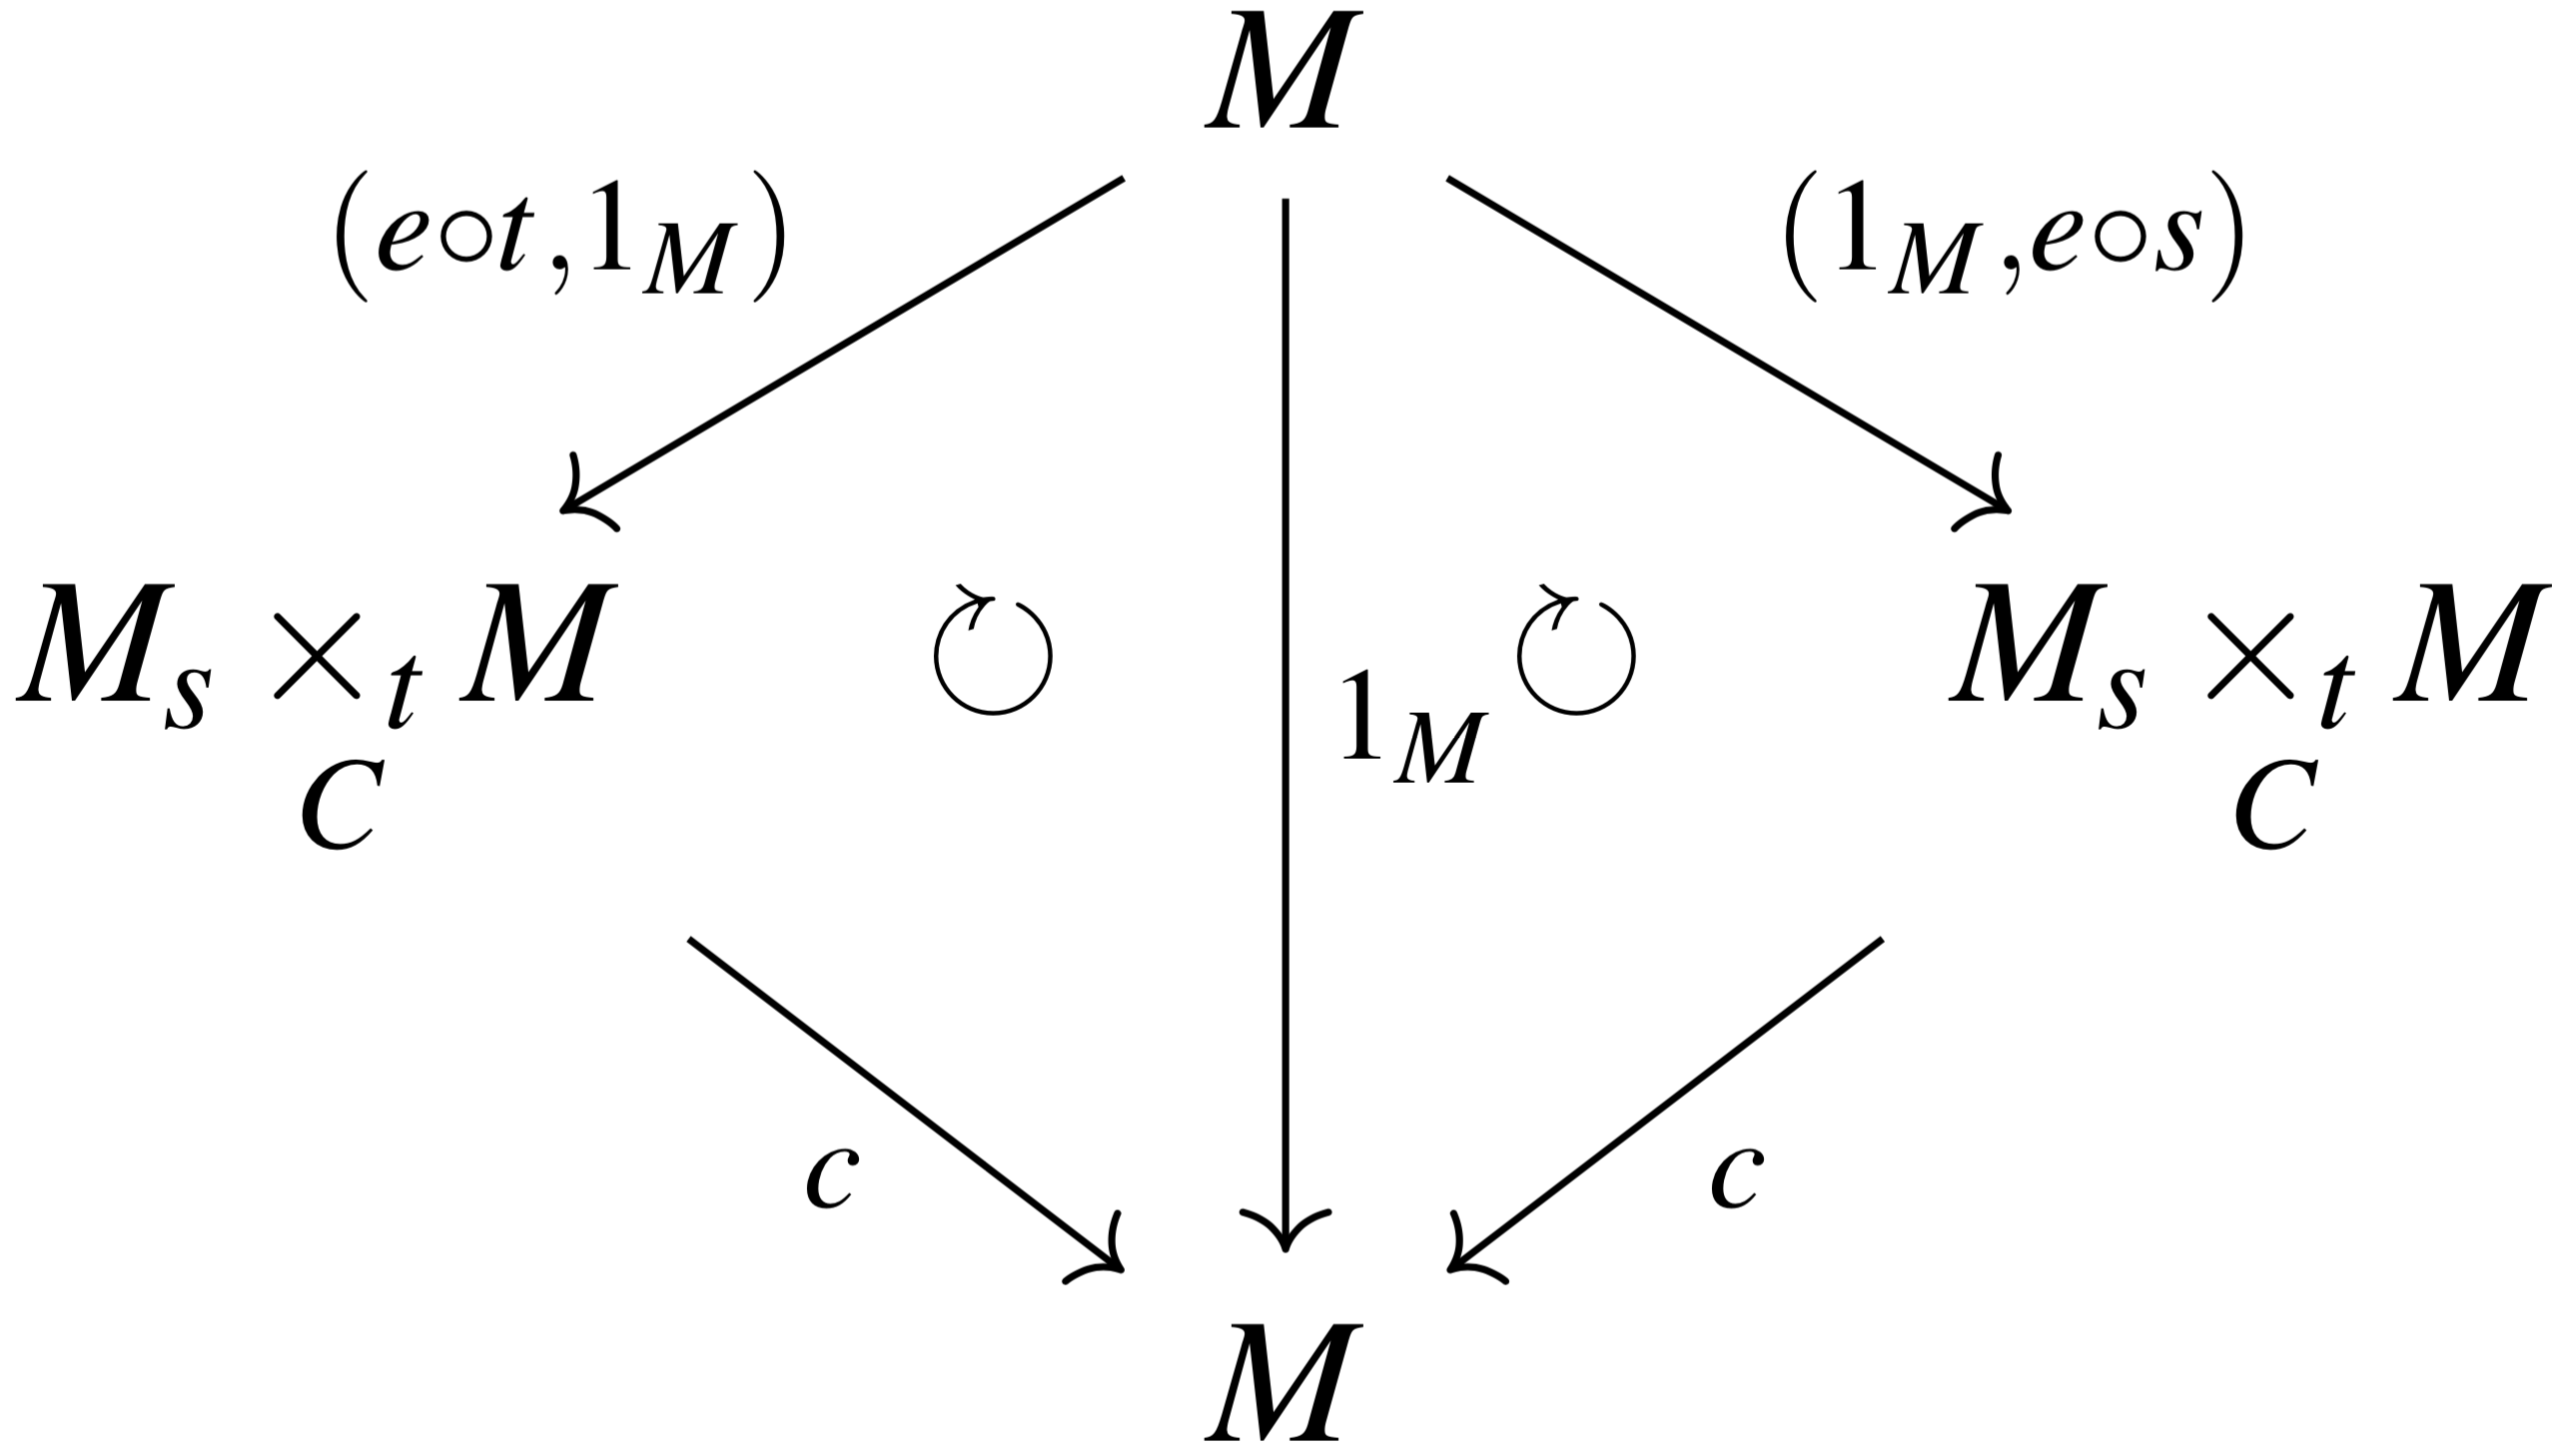
\includegraphics[width=7cm]{cd-4.png}
\end{center}\end{figure}
但し,$e\circ s:M\xrightarrow{\quad s\quad}C\xrightarrow{\quad e \quad}M$であり,
$\begin{array}{ccc}
    (1,e\circ s):M & \longrightarrow & M_s \underset{C}{\times_t}M\\
    \rotatebox{90}{$\in$} & & \rotatebox{90}{$\in$}\\
    f & \longmapsto & (f,e(s(f)))
\end{array}$
である.

\subsection{ここで一息,定義の吟味}

結局,集合論的に言い直せば,$C=ob(\mathcal{C})$,$M=arr(\mathcal{M})$,$s,t$は全ての射に,夫々「始対象」と「終対象」という対象を紐付ける写像$s,t:M\longrightarrow C$,$c$は始対象と終対象が一致する射の組について必ず或る別の射(合成)を対応させる写像$c:M_s \underset{C}{\times_t}M \longrightarrow M$,$e$は対象の一つ一つについて或る射(恒等射)を対応させる写像$e:C\longrightarrow M$(たった一つを選び取る)である.\\
$f\in M$の時,$s(f), t(f)\in C$であるが,この関係を$f:s(f)\longrightarrow t(f)$と書いて(写像の記法と混用.写像も射と見做せるが,射の方が高次元の用語である.),「$f$は$s(f)$から$t(f)$への射である」という.$C$の元である$s(f),t(f)$を以降,夫々アルファベットの大文字で$A,B$などと書くこととする.\\

思うに,「可換」の概念が新しいんだと思う.\\
この定義は,集合論の言葉の上に乗っているが,定義の仕方は極めて圏論的である.写像の情報のみで記述している.(その結果,locally smallな圏のみを圏と定義している.)\\
然し,ということは,理解しやすいように集合論の言葉を援用しているが,このハシゴは外しても圏論自体は崩れないのではないか?つまり,写像と集合はsection1に於いての導入で十分であり,つまり名前を混用しているだけでZFCを背景に仮定する必要もないのではないか?\\
この定義が美しいと思う感覚,今までの集合論的な定義に対して感じていた違和感,どうして圏という概念は洗練されてすでに立派な学問分野になっているのに,定義をするのにこんなに冗長で言葉を浪費するのか?というのは言い出せなかったが兼ねてからの疑問であった.\\
この問題意識の検証を兼ねて,圏論の勉強と数学基礎論の勉強を進めていきたいが,ここではこのまま進んで圏と層について考察する.この定義に出会えたのは後々の跳躍に効いてくるだろう.\\

\noindent
*例えば『層とホモロジー代数』(志甫淳)では,ZFC公理系に,さらに「宇宙の存在公理」を付け加えた公理系で考えている.\\
なるほど,これは逃れられない考え方なのではないか.つまりさ,\\
定義1にて,集合を雑に定義した.これは推移性を明言している.或る推移的集合(これぞ宇宙)の元を集合と以降呼ぶ,と宣言しているのであってさ!\\

\vspace{3mm}
\textbf{定義[Grothendieck universe]}空でない集合$\mathfrak{U}$が宇宙であるとは,以下の4条件を満たすことをいう.\\
1, [推移的集合である]$\forall x,y \; [x\in y \wedge \; y\in \mathfrak{U} \Longrightarrow x\in \mathfrak{U}]$\\
2, [生成規則:pairing]$\forall x,y \; [x,y\in \mathfrak{U} \Longrightarrow \{ x,y\} \in \mathfrak{U}]$\\
3, [生成規則:power]$\forall x \; [x\in\mathfrak{U} \Longrightarrow \mathcal{P}(x):=\{ y:\; y \subset x\} \in \mathfrak{U}]$\\
4, [生成規則:union]$\forall I,x_i \in \mathfrak{U}(i\in I) \; [\; \bigcup_{i\in I} x_i := {y:\; \exists i\in I \; y\in x_i}]$

\textbf{公理[Grothendieck宇宙の存在]}$\mathbb{N}\in\mathcal{U}$を満たす宇宙$\mathcal{U}$が存在する.

\end{document}